\documentclass[1p]{elsarticle_modified}
%\bibliographystyle{elsarticle-num}

%\usepackage[colorlinks]{hyperref}
%\usepackage{abbrmath_seonhwa} %\Abb, \Ascr, \Acal ,\Abf, \Afrak
\usepackage{amsfonts}
\usepackage{amssymb}
\usepackage{amsmath}
\usepackage{amsthm}
\usepackage{scalefnt}
\usepackage{amsbsy}
\usepackage{kotex}
\usepackage{caption}
\usepackage{subfig}
\usepackage{color}
\usepackage{graphicx}
\usepackage{xcolor} %% white, black, red, green, blue, cyan, magenta, yellow
\usepackage{float}
\usepackage{setspace}
\usepackage{hyperref}

\usepackage{tikz}
\usetikzlibrary{arrows}

\usepackage{multirow}
\usepackage{array} % fixed length table
\usepackage{hhline}

%%%%%%%%%%%%%%%%%%%%%
\makeatletter
\renewcommand*\env@matrix[1][\arraystretch]{%
	\edef\arraystretch{#1}%
	\hskip -\arraycolsep
	\let\@ifnextchar\new@ifnextchar
	\array{*\c@MaxMatrixCols c}}
\makeatother %https://tex.stackexchange.com/questions/14071/how-can-i-increase-the-line-spacing-in-a-matrix
%%%%%%%%%%%%%%%

\usepackage[normalem]{ulem}

\newcommand{\msout}[1]{\ifmmode\text{\sout{\ensuremath{#1}}}\else\sout{#1}\fi}
%SOURCE: \msout is \stkout macro in https://tex.stackexchange.com/questions/20609/strikeout-in-math-mode

\newcommand{\cancel}[1]{
	\ifmmode
	{\color{red}\msout{#1}}
	\else
	{\color{red}\sout{#1}}
	\fi
}

\newcommand{\add}[1]{
	{\color{blue}\uwave{#1}}
}

\newcommand{\replace}[2]{
	\ifmmode
	{\color{red}\msout{#1}}{\color{blue}\uwave{#2}}
	\else
	{\color{red}\sout{#1}}{\color{blue}\uwave{#2}}
	\fi
}

\newcommand{\Sol}{\mathcal{S}} %segment
\newcommand{\D}{D} %diagram
\newcommand{\A}{\mathcal{A}} %arc


%%%%%%%%%%%%%%%%%%%%%%%%%%%%%5 test

\def\sl{\operatorname{\textup{SL}}(2,\Cbb)}
\def\psl{\operatorname{\textup{PSL}}(2,\Cbb)}
\def\quan{\mkern 1mu \triangleright \mkern 1mu}

\theoremstyle{definition}
\newtheorem{thm}{Theorem}[section]
\newtheorem{prop}[thm]{Proposition}
\newtheorem{lem}[thm]{Lemma}
\newtheorem{ques}[thm]{Question}
\newtheorem{cor}[thm]{Corollary}
\newtheorem{defn}[thm]{Definition}
\newtheorem{exam}[thm]{Example}
\newtheorem{rmk}[thm]{Remark}
\newtheorem{alg}[thm]{Algorithm}

\newcommand{\I}{\sqrt{-1}}
\begin{document}

%\begin{frontmatter}
%
%\title{Boundary parabolic representations of knots up to 8 crossings}
%
%%% Group authors per affiliation:
%\author{Yunhi Cho} 
%\address{Department of Mathematics, University of Seoul, Seoul, Korea}
%\ead{yhcho@uos.ac.kr}
%
%
%\author{Seonhwa Kim} %\fnref{s_kim}}
%\address{Center for Geometry and Physics, Institute for Basic Science, Pohang, 37673, Korea}
%\ead{ryeona17@ibs.re.kr}
%
%\author{Hyuk Kim}
%\address{Department of Mathematical Sciences, Seoul National University, Seoul 08826, Korea}
%\ead{hyukkim@snu.ac.kr}
%
%\author{Seokbeom Yoon}
%\address{Department of Mathematical Sciences, Seoul National University, Seoul, 08826,  Korea}
%\ead{sbyoon15@snu.ac.kr}
%
%\begin{abstract}
%We find all boundary parabolic representation of knots up to 8 crossings.
%
%\end{abstract}
%\begin{keyword}
%    \MSC[2010] 57M25 
%\end{keyword}
%
%\end{frontmatter}

%\linenumbers
%\tableofcontents
%
\newcommand\colored[1]{\textcolor{white}{\rule[-0.35ex]{0.8em}{1.4ex}}\kern-0.8em\color{red} #1}%
%\newcommand\colored[1]{\textcolor{white}{ #1}\kern-2.17ex	\textcolor{white}{ #1}\kern-1.81ex	\textcolor{white}{ #1}\kern-2.15ex\color{red}#1	}

{\Large $\underline{11n_{50}~(K11n_{50})}$}

\setlength{\tabcolsep}{10pt}
\renewcommand{\arraystretch}{1.6}
\vspace{1cm}\begin{tabular}{m{100pt}>{\centering\arraybackslash}m{274pt}}
\multirow{5}{120pt}{
	\centering
	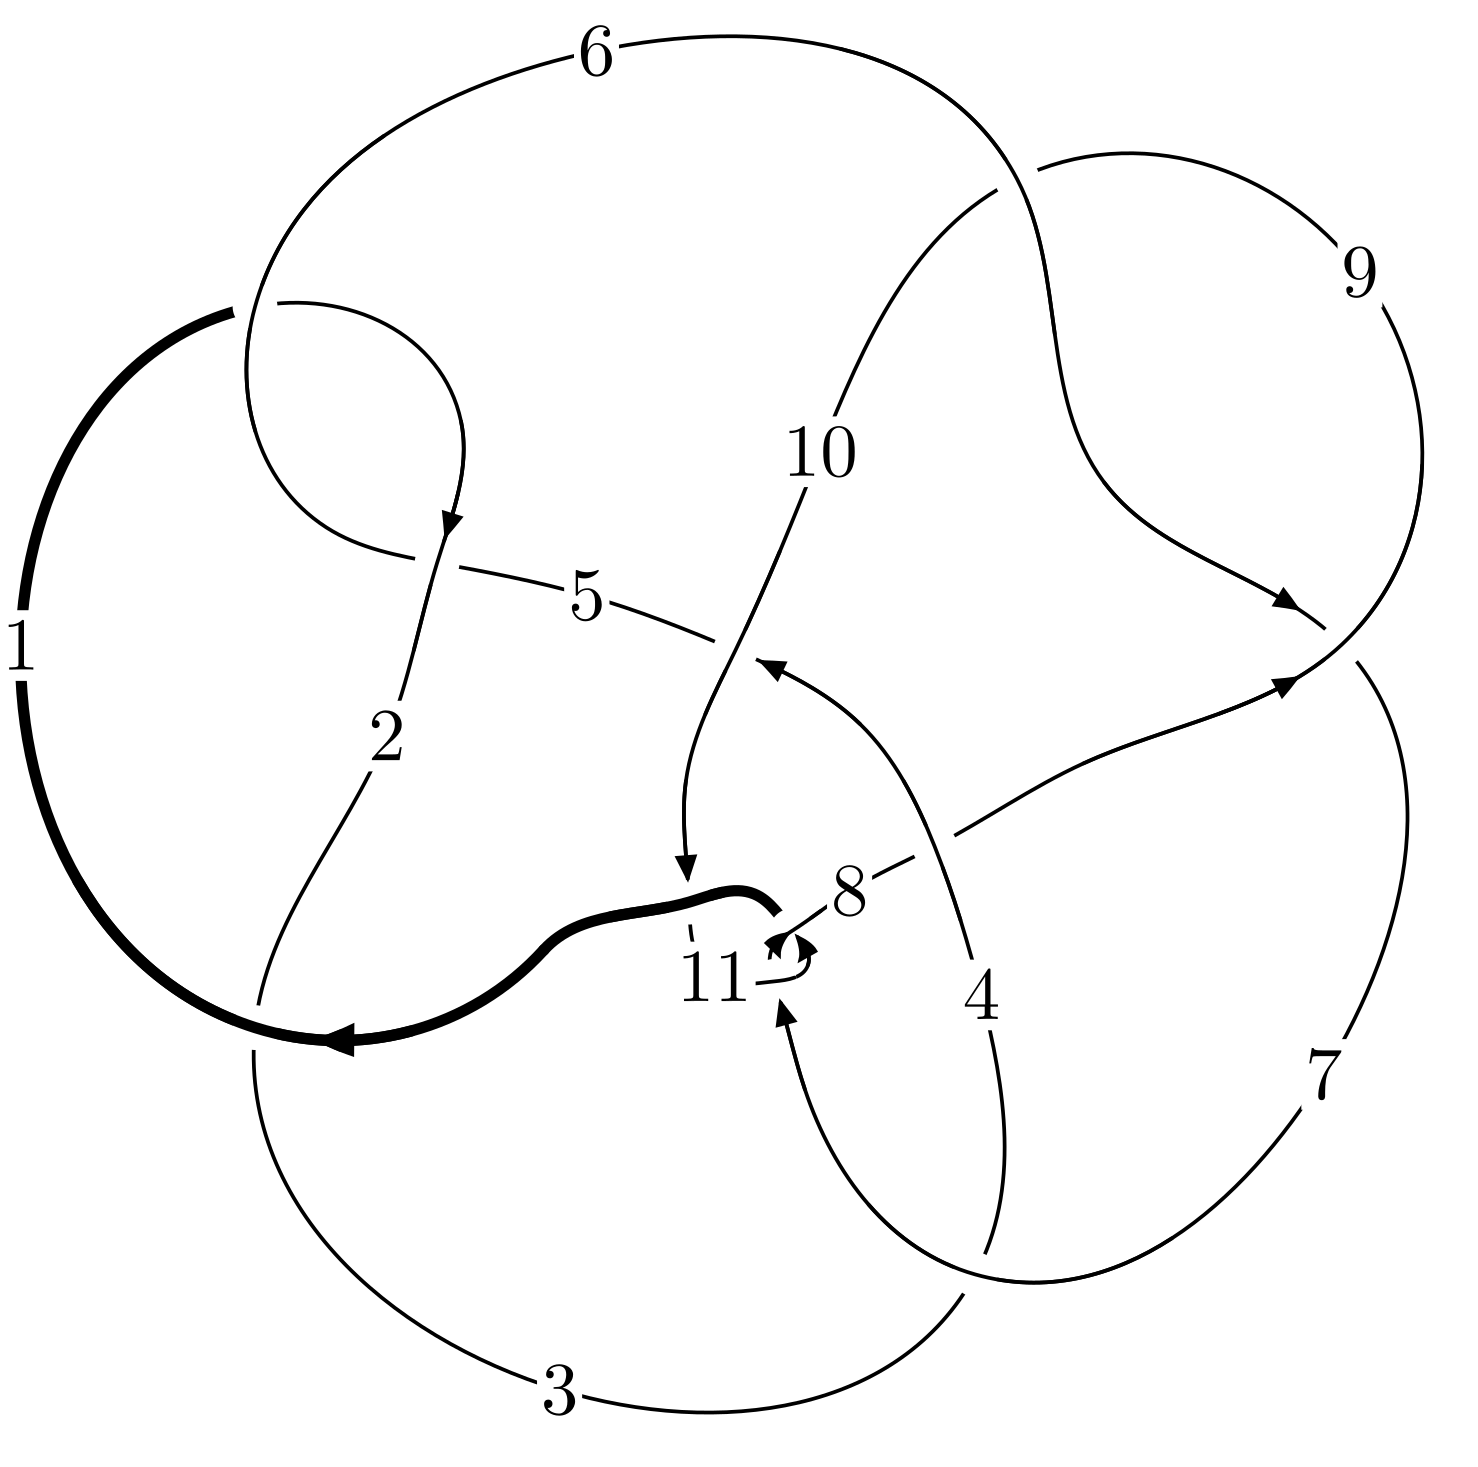
\includegraphics[width=112pt]{../../../GIT/diagram.site/Diagrams/png/666_11n_50.png}\\
\ \ \ A knot diagram\footnotemark}&
\allowdisplaybreaks
\textbf{Linearized knot diagam} \\
\cline{2-2}
 &
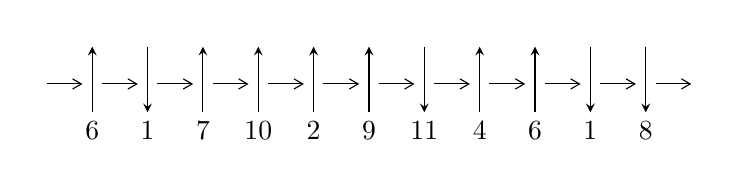
\begin{tikzpicture}[x=20pt, y=17pt]
	% nodes
	\node (C0) at (0, 0) {};
	\node (C1) at (1, 0) {};
	\node (C1U) at (1, +1) {};
	\node (C1D) at (1, -1) {6};

	\node (C2) at (2, 0) {};
	\node (C2U) at (2, +1) {};
	\node (C2D) at (2, -1) {1};

	\node (C3) at (3, 0) {};
	\node (C3U) at (3, +1) {};
	\node (C3D) at (3, -1) {7};

	\node (C4) at (4, 0) {};
	\node (C4U) at (4, +1) {};
	\node (C4D) at (4, -1) {10};

	\node (C5) at (5, 0) {};
	\node (C5U) at (5, +1) {};
	\node (C5D) at (5, -1) {2};

	\node (C6) at (6, 0) {};
	\node (C6U) at (6, +1) {};
	\node (C6D) at (6, -1) {9};

	\node (C7) at (7, 0) {};
	\node (C7U) at (7, +1) {};
	\node (C7D) at (7, -1) {11};

	\node (C8) at (8, 0) {};
	\node (C8U) at (8, +1) {};
	\node (C8D) at (8, -1) {4};

	\node (C9) at (9, 0) {};
	\node (C9U) at (9, +1) {};
	\node (C9D) at (9, -1) {6};

	\node (C10) at (10, 0) {};
	\node (C10U) at (10, +1) {};
	\node (C10D) at (10, -1) {1};

	\node (C11) at (11, 0) {};
	\node (C11U) at (11, +1) {};
	\node (C11D) at (11, -1) {8};
	\node (C12) at (12, 0) {};

	% arrows
	\draw[->,>={angle 60}]
	(C0) edge (C1) (C1) edge (C2) (C2) edge (C3) (C3) edge (C4) (C4) edge (C5) (C5) edge (C6) (C6) edge (C7) (C7) edge (C8) (C8) edge (C9) (C9) edge (C10) (C10) edge (C11) (C11) edge (C12) ;	\draw[->,>=stealth]
	(C1D) edge (C1U) (C2U) edge (C2D) (C3D) edge (C3U) (C4D) edge (C4U) (C5D) edge (C5U) (C6D) edge (C6U) (C7U) edge (C7D) (C8D) edge (C8U) (C9D) edge (C9U) (C10U) edge (C10D) (C11U) edge (C11D) ;
	\end{tikzpicture} \\
\hhline{~~} \\& 
\textbf{Solving Sequence} \\ \cline{2-2} 
 &
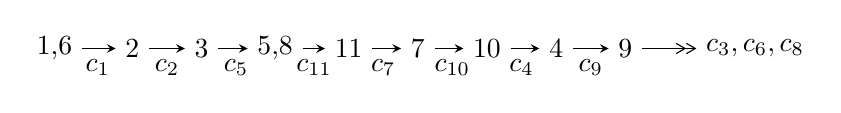
\begin{tikzpicture}[x=25pt, y=7pt]
	% node
	\node (A0) at (-1/8, 0) {1,6};
	\node (A1) at (1, 0) {2};
	\node (A2) at (2, 0) {3};
	\node (A3) at (49/16, 0) {5,8};
	\node (A4) at (33/8, 0) {11};
	\node (A5) at (41/8, 0) {7};
	\node (A6) at (49/8, 0) {10};
	\node (A7) at (57/8, 0) {4};
	\node (A8) at (65/8, 0) {9};
	\node (C1) at (1/2, -1) {$c_{1}$};
	\node (C2) at (3/2, -1) {$c_{2}$};
	\node (C3) at (5/2, -1) {$c_{5}$};
	\node (C4) at (29/8, -1) {$c_{11}$};
	\node (C5) at (37/8, -1) {$c_{7}$};
	\node (C6) at (45/8, -1) {$c_{10}$};
	\node (C7) at (53/8, -1) {$c_{4}$};
	\node (C8) at (61/8, -1) {$c_{9}$};
	\node (A9) at (10, 0) {$c_{3},c_{6},c_{8}$};

	% edge
	\draw[->,>=stealth]	
	(A0) edge (A1) (A1) edge (A2) (A2) edge (A3) (A3) edge (A4) (A4) edge (A5) (A5) edge (A6) (A6) edge (A7) (A7) edge (A8) ;
	\draw[->>,>={angle 60}]	
	(A8) edge (A9);
\end{tikzpicture} \\ 

\end{tabular} \\

\footnotetext{
The image of knot diagram is generated by the software ``\textbf{Draw programme}" developed by Andrew Bartholomew(\url{http://www.layer8.co.uk/maths/draw/index.htm\#Running-draw}), where we modified some parts for our purpose(\url{https://github.com/CATsTAILs/LinksPainter}).
}\phantom \\ \newline 
\centering \textbf{Ideals for irreducible components\footnotemark of $X_{\text{par}}$} 
 
\begin{align*}
I^u_{1}&=\langle 
37910139708041 u^{19}-201150163381549 u^{18}+\cdots+6011452100077376 b-7292662285169845,\\
\phantom{I^u_{1}}&\phantom{= \langle  }-4.50097\times10^{15} u^{19}-1.28986\times10^{16} u^{18}+\cdots+3.00573\times10^{15} a-7.74836\times10^{15},\;u^{20}+3 u^{19}+\cdots+6 u+1\rangle \\
I^u_{2}&=\langle 
- a u+b- u-1,\;a^2-2 a u- u,\;u^2+u+1\rangle \\
I^u_{3}&=\langle 
a u+b+a- u-1,\;a^2-2 a+2,\;u^2+u+1\rangle \\
\\
\end{align*}
\raggedright * 3 irreducible components of $\dim_{\mathbb{C}}=0$, with total 28 representations.\\
\footnotetext{All coefficients of polynomials are rational numbers. But the coefficients are sometimes approximated in decimal forms when there is not enough margin.}
\newpage
\renewcommand{\arraystretch}{1}
\centering \section*{I. $I^u_{1}= \langle 3.79\times10^{13} u^{19}-2.01\times10^{14} u^{18}+\cdots+6.01\times10^{15} b-7.29\times10^{15},\;-4.50\times10^{15} u^{19}-1.29\times10^{16} u^{18}+\cdots+3.01\times10^{15} a-7.75\times10^{15},\;u^{20}+3 u^{19}+\cdots+6 u+1 \rangle$}
\flushleft \textbf{(i) Arc colorings}\\
\begin{tabular}{m{7pt} m{180pt} m{7pt} m{180pt} }
\flushright $a_{1}=$&$\begin{pmatrix}1\\0\end{pmatrix}$ \\
\flushright $a_{6}=$&$\begin{pmatrix}0\\u\end{pmatrix}$ \\
\flushright $a_{2}=$&$\begin{pmatrix}1\\- u^2\end{pmatrix}$ \\
\flushright $a_{3}=$&$\begin{pmatrix}u^2+1\\- u^2\end{pmatrix}$ \\
\flushright $a_{5}=$&$\begin{pmatrix}- u\\u^3+u\end{pmatrix}$ \\
\flushright $a_{8}=$&$\begin{pmatrix}1.49747 u^{19}+4.29134 u^{18}+\cdots+24.6486 u+2.57787\\-0.00630632 u^{19}+0.0334612 u^{18}+\cdots+3.09219 u+1.21313\end{pmatrix}$ \\
\flushright $a_{11}=$&$\begin{pmatrix}-1.01016 u^{19}-2.81974 u^{18}+\cdots-13.1176 u+2.12976\\-0.147188 u^{19}-0.390662 u^{18}+\cdots-5.99436 u-1.23581\end{pmatrix}$ \\
\flushright $a_{7}=$&$\begin{pmatrix}1.20441 u^{19}+3.56367 u^{18}+\cdots+29.2504 u+7.54341\\-0.127524 u^{19}-0.273202 u^{18}+\cdots-3.26181 u+0.411467\end{pmatrix}$ \\
\flushright $a_{10}=$&$\begin{pmatrix}-1.15735 u^{19}-3.21040 u^{18}+\cdots-19.1120 u+0.893945\\-0.147188 u^{19}-0.390662 u^{18}+\cdots-5.99436 u-1.23581\end{pmatrix}$ \\
\flushright $a_{4}=$&$\begin{pmatrix}-1.07688 u^{19}-3.29047 u^{18}+\cdots-25.9886 u-7.95487\\0.115875 u^{19}+0.263182 u^{18}+\cdots+4.66274 u-0.262787\end{pmatrix}$ \\
\flushright $a_{9}=$&$\begin{pmatrix}-1.15735 u^{19}-3.21040 u^{18}+\cdots-19.1120 u+0.893945\\-0.201060 u^{19}-0.575464 u^{18}+\cdots-6.40693 u-1.49747\end{pmatrix}$\\ \flushright $a_{9}=$&$\begin{pmatrix}-1.15735 u^{19}-3.21040 u^{18}+\cdots-19.1120 u+0.893945\\-0.201060 u^{19}-0.575464 u^{18}+\cdots-6.40693 u-1.49747\end{pmatrix}$\\&\end{tabular}
\flushleft \textbf{(ii) Obstruction class $= -1$}\\~\\
\flushleft \textbf{(iii) Cusp Shapes $= \frac{4709825960466509}{3005726050038688} u^{19}+\frac{3061022262562929}{751431512509672} u^{18}+\cdots+\frac{62732012609244425}{3005726050038688} u+\frac{4116636408312339}{751431512509672}$}\\~\\
\newpage\renewcommand{\arraystretch}{1}
\flushleft \textbf{(iv) u-Polynomials at the component}\newline \\
\begin{tabular}{m{50pt}|m{274pt}}
Crossings & \hspace{64pt}u-Polynomials at each crossing \\
\hline $$\begin{aligned}c_{1},c_{5}\end{aligned}$$&$\begin{aligned}
&u^{20}-3 u^{19}+\cdots-6 u+1
\end{aligned}$\\
\hline $$\begin{aligned}c_{2}\end{aligned}$$&$\begin{aligned}
&u^{20}+33 u^{19}+\cdots-6 u+1
\end{aligned}$\\
\hline $$\begin{aligned}c_{3}\end{aligned}$$&$\begin{aligned}
&u^{20}+u^{19}+\cdots+1264 u+517
\end{aligned}$\\
\hline $$\begin{aligned}c_{4}\end{aligned}$$&$\begin{aligned}
&u^{20}+u^{19}+\cdots+1876 u+647
\end{aligned}$\\
\hline $$\begin{aligned}c_{6},c_{9}\end{aligned}$$&$\begin{aligned}
&u^{20}+u^{19}+\cdots+12 u+4
\end{aligned}$\\
\hline $$\begin{aligned}c_{7},c_{11}\end{aligned}$$&$\begin{aligned}
&u^{20}+u^{19}+\cdots+6 u+1
\end{aligned}$\\
\hline $$\begin{aligned}c_{8}\end{aligned}$$&$\begin{aligned}
&u^{20}+u^{19}+\cdots+4 u+1
\end{aligned}$\\
\hline $$\begin{aligned}c_{10}\end{aligned}$$&$\begin{aligned}
&u^{20}+15 u^{19}+\cdots+22 u+1
\end{aligned}$\\
\hline
\end{tabular}\\~\\
\newpage\renewcommand{\arraystretch}{1}
\flushleft \textbf{(v) Riley Polynomials at the component}\newline \\
\begin{tabular}{m{50pt}|m{274pt}}
Crossings & \hspace{64pt}Riley Polynomials at each crossing \\
\hline $$\begin{aligned}c_{1},c_{5}\end{aligned}$$&$\begin{aligned}
&y^{20}+33 y^{19}+\cdots-6 y+1
\end{aligned}$\\
\hline $$\begin{aligned}c_{2}\end{aligned}$$&$\begin{aligned}
&y^{20}-87 y^{19}+\cdots+770 y+1
\end{aligned}$\\
\hline $$\begin{aligned}c_{3}\end{aligned}$$&$\begin{aligned}
&y^{20}+27 y^{19}+\cdots+842544 y+267289
\end{aligned}$\\
\hline $$\begin{aligned}c_{4}\end{aligned}$$&$\begin{aligned}
&y^{20}+55 y^{19}+\cdots-892556 y+418609
\end{aligned}$\\
\hline $$\begin{aligned}c_{6},c_{9}\end{aligned}$$&$\begin{aligned}
&y^{20}+33 y^{19}+\cdots-120 y+16
\end{aligned}$\\
\hline $$\begin{aligned}c_{7},c_{11}\end{aligned}$$&$\begin{aligned}
&y^{20}-15 y^{19}+\cdots-22 y+1
\end{aligned}$\\
\hline $$\begin{aligned}c_{8}\end{aligned}$$&$\begin{aligned}
&y^{20}-3 y^{19}+\cdots-6 y+1
\end{aligned}$\\
\hline $$\begin{aligned}c_{10}\end{aligned}$$&$\begin{aligned}
&y^{20}-15 y^{19}+\cdots+50 y+1
\end{aligned}$\\
\hline
\end{tabular}\\~\\
\newpage\flushleft \textbf{(vi) Complex Volumes and Cusp Shapes}
$$\begin{array}{c|c|c}  
\text{Solutions to }I^u_{1}& \I (\text{vol} + \sqrt{-1}CS) & \text{Cusp shape}\\
 \hline 
\begin{aligned}
u &= -0.562478 + 0.702926 I \\
a &= -0.164935 + 1.014010 I \\
b &= -0.932716 - 0.491902 I\end{aligned}
 & \phantom{-}0.10443 - 4.15417 I & \phantom{-}5.96079 + 7.41844 I \\ \hline\begin{aligned}
u &= -0.562478 - 0.702926 I \\
a &= -0.164935 - 1.014010 I \\
b &= -0.932716 + 0.491902 I\end{aligned}
 & \phantom{-}0.10443 + 4.15417 I & \phantom{-}5.96079 - 7.41844 I \\ \hline\begin{aligned}
u &= -0.345261 + 0.774594 I \\
a &= -0.178688 + 1.067020 I \\
b &= \phantom{-}0.262517 + 0.119217 I\end{aligned}
 & -1.78458 - 2.08707 I & -0.67504 + 3.91538 I \\ \hline\begin{aligned}
u &= -0.345261 - 0.774594 I \\
a &= -0.178688 - 1.067020 I \\
b &= \phantom{-}0.262517 - 0.119217 I\end{aligned}
 & -1.78458 + 2.08707 I & -0.67504 - 3.91538 I \\ \hline\begin{aligned}
u &= -0.546407 + 0.261165 I \\
a &= -0.016518 - 0.458675 I \\
b &= -0.503419 + 0.405661 I\end{aligned}
 & \phantom{-}1.204440 - 0.232928 I & \phantom{-}9.01931 + 0.79005 I \\ \hline\begin{aligned}
u &= -0.546407 - 0.261165 I \\
a &= -0.016518 + 0.458675 I \\
b &= -0.503419 - 0.405661 I\end{aligned}
 & \phantom{-}1.204440 + 0.232928 I & \phantom{-}9.01931 - 0.79005 I \\ \hline\begin{aligned}
u &= \phantom{-}0.55309 + 1.41617 I \\
a &= \phantom{-}0.152667 - 0.289034 I \\
b &= -1.369770 - 0.179262 I\end{aligned}
 & -7.00299 - 3.90150 I & -2.54860 + 3.27736 I \\ \hline\begin{aligned}
u &= \phantom{-}0.55309 - 1.41617 I \\
a &= \phantom{-}0.152667 + 0.289034 I \\
b &= -1.369770 + 0.179262 I\end{aligned}
 & -7.00299 + 3.90150 I & -2.54860 - 3.27736 I \\ \hline\begin{aligned}
u &= \phantom{-}0.368558 + 0.047969 I \\
a &= -1.78216 + 1.81771 I \\
b &= \phantom{-}1.053190 - 0.370537 I\end{aligned}
 & -1.82190 + 1.34830 I & -1.59816 - 0.61194 I \\ \hline\begin{aligned}
u &= \phantom{-}0.368558 - 0.047969 I \\
a &= -1.78216 - 1.81771 I \\
b &= \phantom{-}1.053190 + 0.370537 I\end{aligned}
 & -1.82190 - 1.34830 I & -1.59816 + 0.61194 I\\
 \hline 
 \end{array}$$\newpage$$\begin{array}{c|c|c}  
\text{Solutions to }I^u_{1}& \I (\text{vol} + \sqrt{-1}CS) & \text{Cusp shape}\\
 \hline 
\begin{aligned}
u &= -0.140514 + 0.165365 I \\
a &= -1.96129 + 4.14993 I \\
b &= \phantom{-}0.715874 + 0.509667 I\end{aligned}
 & -1.42072 - 2.15124 I & \phantom{-}1.64791 + 3.40317 I \\ \hline\begin{aligned}
u &= -0.140514 - 0.165365 I \\
a &= -1.96129 - 4.14993 I \\
b &= \phantom{-}0.715874 - 0.509667 I\end{aligned}
 & -1.42072 + 2.15124 I & \phantom{-}1.64791 - 3.40317 I \\ \hline\begin{aligned}
u &= -0.93727 + 1.53815 I \\
a &= -0.097983 - 0.641269 I \\
b &= \phantom{-}1.281060 + 0.067311 I\end{aligned}
 & -5.23226 - 2.45917 I & -1.69714 + 1.89268 I \\ \hline\begin{aligned}
u &= -0.93727 - 1.53815 I \\
a &= -0.097983 + 0.641269 I \\
b &= \phantom{-}1.281060 - 0.067311 I\end{aligned}
 & -5.23226 + 2.45917 I & -1.69714 - 1.89268 I \\ \hline\begin{aligned}
u &= -0.00083 + 2.05851 I \\
a &= -0.027063 + 1.246070 I \\
b &= \phantom{-}0.076044 - 1.204780 I\end{aligned}
 & -13.59470 - 3.72129 I & \phantom{-}0.72655 + 1.99965 I \\ \hline\begin{aligned}
u &= -0.00083 - 2.05851 I \\
a &= -0.027063 - 1.246070 I \\
b &= \phantom{-}0.076044 + 1.204780 I\end{aligned}
 & -13.59470 + 3.72129 I & \phantom{-}0.72655 - 1.99965 I \\ \hline\begin{aligned}
u &= \phantom{-}0.48389 + 2.08874 I \\
a &= \phantom{-}0.342044 - 1.052760 I \\
b &= -1.48289 + 0.54439 I\end{aligned}
 & -18.5347 + 2.5424 I & -1.82827 + 0. I\phantom{ +0.000000I} \\ \hline\begin{aligned}
u &= \phantom{-}0.48389 - 2.08874 I \\
a &= \phantom{-}0.342044 + 1.052760 I \\
b &= -1.48289 - 0.54439 I\end{aligned}
 & -18.5347 - 2.5424 I & -1.82827 + 0. I\phantom{ +0.000000I} \\ \hline\begin{aligned}
u &= -0.37279 + 2.18713 I \\
a &= -0.266075 - 1.115660 I \\
b &= \phantom{-}1.40011 + 0.62778 I\end{aligned}
 & -17.7144 - 10.2068 I & \phantom{-0.000000 -}0. + 4.81283 I \\ \hline\begin{aligned}
u &= -0.37279 - 2.18713 I \\
a &= -0.266075 + 1.115660 I \\
b &= \phantom{-}1.40011 - 0.62778 I\end{aligned}
 & -17.7144 + 10.2068 I & \phantom{-0.000000 } 0. - 4.81283 I\\
 \hline 
 \end{array}$$\newpage\newpage\renewcommand{\arraystretch}{1}
\centering \section*{II. $I^u_{2}= \langle - a u+b- u-1,\;a^2-2 a u- u,\;u^2+u+1 \rangle$}
\flushleft \textbf{(i) Arc colorings}\\
\begin{tabular}{m{7pt} m{180pt} m{7pt} m{180pt} }
\flushright $a_{1}=$&$\begin{pmatrix}1\\0\end{pmatrix}$ \\
\flushright $a_{6}=$&$\begin{pmatrix}0\\u\end{pmatrix}$ \\
\flushright $a_{2}=$&$\begin{pmatrix}1\\u+1\end{pmatrix}$ \\
\flushright $a_{3}=$&$\begin{pmatrix}- u\\u+1\end{pmatrix}$ \\
\flushright $a_{5}=$&$\begin{pmatrix}- u\\u+1\end{pmatrix}$ \\
\flushright $a_{8}=$&$\begin{pmatrix}a\\a u+u+1\end{pmatrix}$ \\
\flushright $a_{11}=$&$\begin{pmatrix}a u+a+u+2\\- u-1\end{pmatrix}$ \\
\flushright $a_{7}=$&$\begin{pmatrix}u+1\\a u+a+1\end{pmatrix}$ \\
\flushright $a_{10}=$&$\begin{pmatrix}a u+a+1\\- u-1\end{pmatrix}$ \\
\flushright $a_{4}=$&$\begin{pmatrix}- a u- a- u-2\\- a+3 u+2\end{pmatrix}$ \\
\flushright $a_{9}=$&$\begin{pmatrix}a u+a+1\\- a u-2 u-2\end{pmatrix}$\\ \flushright $a_{9}=$&$\begin{pmatrix}a u+a+1\\- a u-2 u-2\end{pmatrix}$\\&\end{tabular}
\flushleft \textbf{(ii) Obstruction class $= 1$}\\~\\
\flushleft \textbf{(iii) Cusp Shapes $= 8 u+4$}\\~\\
\newpage\renewcommand{\arraystretch}{1}
\flushleft \textbf{(iv) u-Polynomials at the component}\newline \\
\begin{tabular}{m{50pt}|m{274pt}}
Crossings & \hspace{64pt}u-Polynomials at each crossing \\
\hline $$\begin{aligned}c_{1},c_{2}\end{aligned}$$&$\begin{aligned}
&(u^2+u+1)^2
\end{aligned}$\\
\hline $$\begin{aligned}c_{3}\end{aligned}$$&$\begin{aligned}
&u^4-2 u^3+5 u^2-4 u+1
\end{aligned}$\\
\hline $$\begin{aligned}c_{4}\end{aligned}$$&$\begin{aligned}
&u^4+4 u^3+5 u^2+2 u+1
\end{aligned}$\\
\hline $$\begin{aligned}c_{5},c_{10}\end{aligned}$$&$\begin{aligned}
&(u^2- u+1)^2
\end{aligned}$\\
\hline $$\begin{aligned}c_{6},c_{9}\end{aligned}$$&$\begin{aligned}
&(u^2+1)^2
\end{aligned}$\\
\hline $$\begin{aligned}c_{7},c_{8},c_{11}\end{aligned}$$&$\begin{aligned}
&u^4- u^2+1
\end{aligned}$\\
\hline
\end{tabular}\\~\\
\newpage\renewcommand{\arraystretch}{1}
\flushleft \textbf{(v) Riley Polynomials at the component}\newline \\
\begin{tabular}{m{50pt}|m{274pt}}
Crossings & \hspace{64pt}Riley Polynomials at each crossing \\
\hline $$\begin{aligned}c_{1},c_{2},c_{5}\\c_{10}\end{aligned}$$&$\begin{aligned}
&(y^2+y+1)^2
\end{aligned}$\\
\hline $$\begin{aligned}c_{3}\end{aligned}$$&$\begin{aligned}
&y^4+6 y^3+11 y^2-6 y+1
\end{aligned}$\\
\hline $$\begin{aligned}c_{4}\end{aligned}$$&$\begin{aligned}
&y^4-6 y^3+11 y^2+6 y+1
\end{aligned}$\\
\hline $$\begin{aligned}c_{6},c_{9}\end{aligned}$$&$\begin{aligned}
&(y+1)^4
\end{aligned}$\\
\hline $$\begin{aligned}c_{7},c_{8},c_{11}\end{aligned}$$&$\begin{aligned}
&(y^2- y+1)^2
\end{aligned}$\\
\hline
\end{tabular}\\~\\
\newpage\flushleft \textbf{(vi) Complex Volumes and Cusp Shapes}
$$\begin{array}{c|c|c}  
\text{Solutions to }I^u_{2}& \I (\text{vol} + \sqrt{-1}CS) & \text{Cusp shape}\\
 \hline 
\begin{aligned}
u &= -0.500000 + 0.866025 I \\
a &= -0.500000 - 0.133975 I \\
b &= \phantom{-}0.866025 + 0.500000 I\end{aligned}
 & -1.64493 - 4.05977 I & \phantom{-0.000000 -}0. + 6.92820 I \\ \hline\begin{aligned}
u &= -0.500000 + 0.866025 I \\
a &= -0.50000 + 1.86603 I \\
b &= -0.866025 - 0.500000 I\end{aligned}
 & -1.64493 - 4.05977 I & \phantom{-0.000000 -}0. + 6.92820 I \\ \hline\begin{aligned}
u &= -0.500000 - 0.866025 I \\
a &= -0.500000 + 0.133975 I \\
b &= \phantom{-}0.866025 - 0.500000 I\end{aligned}
 & -1.64493 + 4.05977 I & \phantom{-0.000000 } 0. - 6.92820 I \\ \hline\begin{aligned}
u &= -0.500000 - 0.866025 I \\
a &= -0.50000 - 1.86603 I \\
b &= -0.866025 + 0.500000 I\end{aligned}
 & -1.64493 + 4.05977 I & \phantom{-0.000000 } 0. - 6.92820 I\\
 \hline 
 \end{array}$$\newpage\newpage\renewcommand{\arraystretch}{1}
\centering \section*{III. $I^u_{3}= \langle a u+b+a- u-1,\;a^2-2 a+2,\;u^2+u+1 \rangle$}
\flushleft \textbf{(i) Arc colorings}\\
\begin{tabular}{m{7pt} m{180pt} m{7pt} m{180pt} }
\flushright $a_{1}=$&$\begin{pmatrix}1\\0\end{pmatrix}$ \\
\flushright $a_{6}=$&$\begin{pmatrix}0\\u\end{pmatrix}$ \\
\flushright $a_{2}=$&$\begin{pmatrix}1\\u+1\end{pmatrix}$ \\
\flushright $a_{3}=$&$\begin{pmatrix}- u\\u+1\end{pmatrix}$ \\
\flushright $a_{5}=$&$\begin{pmatrix}- u\\u+1\end{pmatrix}$ \\
\flushright $a_{8}=$&$\begin{pmatrix}a\\- a u- a+u+1\end{pmatrix}$ \\
\flushright $a_{11}=$&$\begin{pmatrix}a u+a-2 u-1\\u\end{pmatrix}$ \\
\flushright $a_{7}=$&$\begin{pmatrix}u+1\\- a u+u\end{pmatrix}$ \\
\flushright $a_{10}=$&$\begin{pmatrix}a u+a- u-1\\u\end{pmatrix}$ \\
\flushright $a_{4}=$&$\begin{pmatrix}a u-2 u-1\\a u+a-1\end{pmatrix}$ \\
\flushright $a_{9}=$&$\begin{pmatrix}a u+a- u-1\\- a u+2 u\end{pmatrix}$\\ \flushright $a_{9}=$&$\begin{pmatrix}a u+a- u-1\\- a u+2 u\end{pmatrix}$\\&\end{tabular}
\flushleft \textbf{(ii) Obstruction class $= 1$}\\~\\
\flushleft \textbf{(iii) Cusp Shapes $= 0$}\\~\\
\newpage\renewcommand{\arraystretch}{1}
\flushleft \textbf{(iv) u-Polynomials at the component}\newline \\
\begin{tabular}{m{50pt}|m{274pt}}
Crossings & \hspace{64pt}u-Polynomials at each crossing \\
\hline $$\begin{aligned}c_{1},c_{2}\end{aligned}$$&$\begin{aligned}
&(u^2+u+1)^2
\end{aligned}$\\
\hline $$\begin{aligned}c_{3},c_{4}\end{aligned}$$&$\begin{aligned}
&u^4-2 u^3+2 u^2+2 u+1
\end{aligned}$\\
\hline $$\begin{aligned}c_{5},c_{10}\end{aligned}$$&$\begin{aligned}
&(u^2- u+1)^2
\end{aligned}$\\
\hline $$\begin{aligned}c_{6},c_{9}\end{aligned}$$&$\begin{aligned}
&(u^2+1)^2
\end{aligned}$\\
\hline $$\begin{aligned}c_{7},c_{8},c_{11}\end{aligned}$$&$\begin{aligned}
&u^4- u^2+1
\end{aligned}$\\
\hline
\end{tabular}\\~\\
\newpage\renewcommand{\arraystretch}{1}
\flushleft \textbf{(v) Riley Polynomials at the component}\newline \\
\begin{tabular}{m{50pt}|m{274pt}}
Crossings & \hspace{64pt}Riley Polynomials at each crossing \\
\hline $$\begin{aligned}c_{1},c_{2},c_{5}\\c_{10}\end{aligned}$$&$\begin{aligned}
&(y^2+y+1)^2
\end{aligned}$\\
\hline $$\begin{aligned}c_{3},c_{4}\end{aligned}$$&$\begin{aligned}
&y^4+14 y^2+1
\end{aligned}$\\
\hline $$\begin{aligned}c_{6},c_{9}\end{aligned}$$&$\begin{aligned}
&(y+1)^4
\end{aligned}$\\
\hline $$\begin{aligned}c_{7},c_{8},c_{11}\end{aligned}$$&$\begin{aligned}
&(y^2- y+1)^2
\end{aligned}$\\
\hline
\end{tabular}\\~\\
\newpage\flushleft \textbf{(vi) Complex Volumes and Cusp Shapes}
$$\begin{array}{c|c|c}  
\text{Solutions to }I^u_{3}& \I (\text{vol} + \sqrt{-1}CS) & \text{Cusp shape}\\
 \hline 
\begin{aligned}
u &= -0.500000 + 0.866025 I \\
a &= \phantom{-}1.00000 + 1.00000 I \\
b &= \phantom{-}0.866025 - 0.500000 I\end{aligned}
 & -1.64493\phantom{ +0.000000I} & \phantom{-0.000000 } 0 \\ \hline\begin{aligned}
u &= -0.500000 + 0.866025 I \\
a &= \phantom{-}1.00000 - 1.00000 I \\
b &= -0.866025 + 0.500000 I\end{aligned}
 & -1.64493\phantom{ +0.000000I} & \phantom{-0.000000 } 0 \\ \hline\begin{aligned}
u &= -0.500000 - 0.866025 I \\
a &= \phantom{-}1.00000 + 1.00000 I \\
b &= -0.866025 - 0.500000 I\end{aligned}
 & -1.64493\phantom{ +0.000000I} & \phantom{-0.000000 } 0 \\ \hline\begin{aligned}
u &= -0.500000 - 0.866025 I \\
a &= \phantom{-}1.00000 - 1.00000 I \\
b &= \phantom{-}0.866025 + 0.500000 I\end{aligned}
 & -1.64493\phantom{ +0.000000I} & \phantom{-0.000000 } 0\\
 \hline 
 \end{array}$$\newpage
\newpage\renewcommand{\arraystretch}{1}
\centering \section*{ IV. u-Polynomials}
\begin{tabular}{m{50pt}|m{274pt}}
Crossings & \hspace{64pt}u-Polynomials at each crossing \\
\hline $$\begin{aligned}c_{1}\end{aligned}$$&$\begin{aligned}
&((u^2+u+1)^4)(u^{20}-3 u^{19}+\cdots-6 u+1)
\end{aligned}$\\
\hline $$\begin{aligned}c_{2}\end{aligned}$$&$\begin{aligned}
&((u^2+u+1)^4)(u^{20}+33 u^{19}+\cdots-6 u+1)
\end{aligned}$\\
\hline $$\begin{aligned}c_{3}\end{aligned}$$&$\begin{aligned}
&(u^4-2 u^3+2 u^2+2 u+1)(u^4-2 u^3+5 u^2-4 u+1)\\
&\cdot(u^{20}+u^{19}+\cdots+1264 u+517)
\end{aligned}$\\
\hline $$\begin{aligned}c_{4}\end{aligned}$$&$\begin{aligned}
&(u^4-2 u^3+2 u^2+2 u+1)(u^4+4 u^3+5 u^2+2 u+1)\\
&\cdot(u^{20}+u^{19}+\cdots+1876 u+647)
\end{aligned}$\\
\hline $$\begin{aligned}c_{5}\end{aligned}$$&$\begin{aligned}
&((u^2- u+1)^4)(u^{20}-3 u^{19}+\cdots-6 u+1)
\end{aligned}$\\
\hline $$\begin{aligned}c_{6},c_{9}\end{aligned}$$&$\begin{aligned}
&((u^2+1)^4)(u^{20}+u^{19}+\cdots+12 u+4)
\end{aligned}$\\
\hline $$\begin{aligned}c_{7},c_{11}\end{aligned}$$&$\begin{aligned}
&((u^4- u^2+1)^2)(u^{20}+u^{19}+\cdots+6 u+1)
\end{aligned}$\\
\hline $$\begin{aligned}c_{8}\end{aligned}$$&$\begin{aligned}
&((u^4- u^2+1)^2)(u^{20}+u^{19}+\cdots+4 u+1)
\end{aligned}$\\
\hline $$\begin{aligned}c_{10}\end{aligned}$$&$\begin{aligned}
&((u^2- u+1)^4)(u^{20}+15 u^{19}+\cdots+22 u+1)
\end{aligned}$\\
\hline
\end{tabular}\newpage\renewcommand{\arraystretch}{1}
\centering \section*{ V. Riley Polynomials}
\begin{tabular}{m{50pt}|m{274pt}}
Crossings & \hspace{64pt}Riley Polynomials at each crossing \\
\hline $$\begin{aligned}c_{1},c_{5}\end{aligned}$$&$\begin{aligned}
&((y^2+y+1)^4)(y^{20}+33 y^{19}+\cdots-6 y+1)
\end{aligned}$\\
\hline $$\begin{aligned}c_{2}\end{aligned}$$&$\begin{aligned}
&((y^2+y+1)^4)(y^{20}-87 y^{19}+\cdots+770 y+1)
\end{aligned}$\\
\hline $$\begin{aligned}c_{3}\end{aligned}$$&$\begin{aligned}
&(y^4+14 y^2+1)(y^4+6 y^3+11 y^2-6 y+1)\\
&\cdot(y^{20}+27 y^{19}+\cdots+842544 y+267289)
\end{aligned}$\\
\hline $$\begin{aligned}c_{4}\end{aligned}$$&$\begin{aligned}
&(y^4+14 y^2+1)(y^4-6 y^3+11 y^2+6 y+1)\\
&\cdot(y^{20}+55 y^{19}+\cdots-892556 y+418609)
\end{aligned}$\\
\hline $$\begin{aligned}c_{6},c_{9}\end{aligned}$$&$\begin{aligned}
&((y+1)^8)(y^{20}+33 y^{19}+\cdots-120 y+16)
\end{aligned}$\\
\hline $$\begin{aligned}c_{7},c_{11}\end{aligned}$$&$\begin{aligned}
&((y^2- y+1)^4)(y^{20}-15 y^{19}+\cdots-22 y+1)
\end{aligned}$\\
\hline $$\begin{aligned}c_{8}\end{aligned}$$&$\begin{aligned}
&((y^2- y+1)^4)(y^{20}-3 y^{19}+\cdots-6 y+1)
\end{aligned}$\\
\hline $$\begin{aligned}c_{10}\end{aligned}$$&$\begin{aligned}
&((y^2+y+1)^4)(y^{20}-15 y^{19}+\cdots+50 y+1)
\end{aligned}$\\
\hline
\end{tabular}
\vskip 2pc
\end{document}